
Since the system is to be able to run on two different platforms, the hardware requirements differ a lot depending on which system being considered. In the case of Raspberry Pi computers being used, all cameras each have their own Raspberry Pi processing unit where image processing takes place. In case of a central image processing unit (laptop, server or desktop computer), image processing from all cameras in the room take place on this central unit.


\begin{figure}[htb]
	\centering
	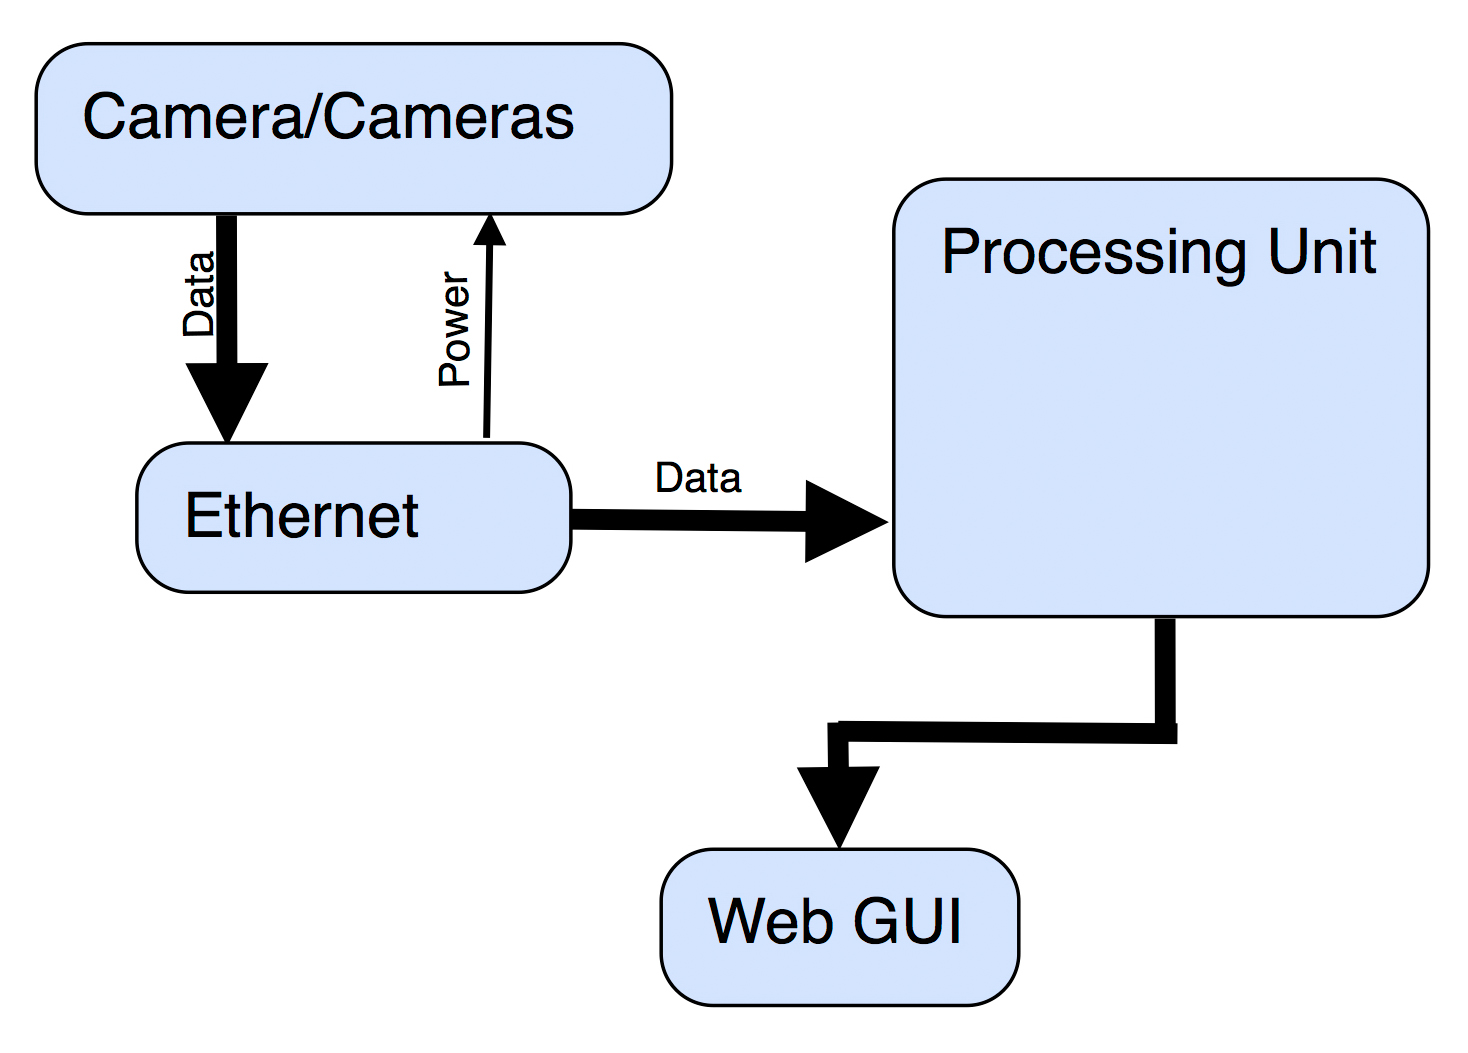
\includegraphics[width=160mm]{images/Hardware-flowchart.jpg}
	\caption[This text ends up at the list of figures]{\textit{Flowchart hardware modules}}
	\label{fig:block_overview_fig}  %Skapar referens till figuren
\end{figure}


\subsection{Limitations}
The hardware is limited by budget, Internet connection and the source of power. The cost is limited to approximately 15.000 SEK per room, including installation costs. The budget limits performance of the cameras e.g. resolution and number of cameras. The connection to the cameras need to be stable and have a bandwidth good enough for sending live video from the cameras.   
\newpage
\subsection{Hardware Requirements}
\label{sec:hardware_req}
\reqtable
{
	\addreq{The system uses network cameras powered via Ethernet.\newline \textbf{Revised 2013-11-27:} The system uses cameras connected to a laptop (mid-end processing device) via network or USB.}{1}	
	\addreq{The system can operate using high resolution ($>$1 Mpixel) cameras}{1}
	\addreq{Lower resolution cameras can be used}{2}
	\addreq{The application can run using the processing power provided by the costumer.\newline \textbf{Canceled 2013-11-27: }No processing power is provided by the customer.}{--}
	\addreq{The application can run using a mid-end processing device.\newline \textbf{Revised priority 2013-11-27:} The cancellation of previous req.(\textbf{3.4}) causes priority to change \textbf{from 2 to 1.}}{1}
	\addreq{The application can run using a low-end processing device.\newline	\textbf{Revised priority 2013-11-27:} Revised due to a request from customer that the system is able to run on a Raspberry Pi. Priority changed \textbf{from 3 to 2.}}{2}
}